
\documentclass[12pt,usenames,dvipsnames]{iopart}
\newcommand{\gguide}{{\it Preparing graphics for IOP Publishing journals}}

\usepackage[a4paper=false,
            citecolor=blue,
            colorlinks=true,
            urlcolor=blue,
            linkcolor=blue,
            pdfauthor={Prannaya Gupta},
            pdftitle={Deployment of Dionaea and ElasticHoney Honeypots using the MHN},
            pdfsubject={Deployment of Dionaea and ElasticHoney Honeypots using the MHN},
            pdfkeywords={honeypot, cybersecurity}
            ]{hyperref}
\usepackage{graphicx}
\usepackage{parskip}
\usepackage{caption}
\usepackage{subcaption}
\usepackage{soul}
\usepackage{booktabs}
\usepackage{tcolorbox}

\usepackage{algorithm}
\usepackage{algpseudocode}

\usepackage{menukeys} 


% \usepackage[usenames,dvipsnames]{color}


\newcommand*{\thead}[1]{%
\multicolumn{1}{c}{\bfseries\begin{tabular}{@{}c@{}}#1\end{tabular}}}

\newcommand{\reftable}[1]{\hyperref[#1]{Table \ref*{#1}}}
\newcommand{\reffig}[1]{\hyperref[#1]{Figure \ref*{#1}}}
\newcommand{\refalgo}[1]{\hyperref[#1]{Algorithm \ref*{#1}}}

\begin{document}

\title[Deployment of Dionaea and ElasticHoney Honeypots using the MHN]{\st{money} honey is all you need: Deployment of Dionaea and ElasticHoney Honeypots using the Modern Honeypot Network (MHN)}

% \author{Prannaya Gupta (M23604)}

% \address{Department of Computer Science, NUS High School of Mathematics and Science, 20 Clementi Ave 1, 129957, Singapore}
% \ead{\href{mailto:h1810124@nushigh.edu.sg}{h1810124@nushigh.edu.sg}}
% \vspace{10pt}
% \begin{indented}
% \item[]August 2023
% \end{indented}
\setlength{\parskip}{6pt}
\setlength{\parindent}{25pt}

% \begin{abstract}
% insert abstract here

% \noindent{Keywords}: honeypot, cloud computing, Google Cloud Platform, virtual machines, firewall, deception, cybersecurity
% \end{abstract}

% \submitto{\PS}

\section{Introduction} \label{sec-intro}

A \emph{honeypot network} is a simple mechanism adapted by various companies that exists simply to be compromised. An attack on a honeypot is effectively a trap, where, whilst the attacker believes that they are compromising a system, they are simply letting the trap record their personal details \cite{spitzner2003honeynet}. Honeypots are often used to identify hints to the source and size of attacks, and also become an invaluable source of malicious and exploitative software.



\section{Background} \label{sec-background}

There are several different honeypots that try to achieve different goals.

\textbf{Cowrie} is an example of a very basic SSH honeypot. A SSH honeypot behaves similarly to a virtual machine where in someone tries to access the VM and a mock console interface is displayed. This console interface is controlled centrally by a server and it basically replicates the console interface expected in a common user interface.

\textbf{Dionaea} \cite{visoottiviseth2011distributed} is a malware-capturing honeypot that was developed under Google Summer of Code (GSoC) 2009 via the The Honeynet Project. This honeypot uses various connection systems to capture malware files. 

Due to restrictions of time and resources, among other reasons, we have decided to test the Dionaea architecture.

\section{Methodology} \label{sec-methodology}

In this work, we use the \href{https://github.com/CSIRT-UMM/mhn}{\textbf{Modern Honeypot Network (MHN)}}, or rather a variation suited for \texttt{Ubuntu 20.04}. We deploy this service onto the Google Cloud Platform (GCP) for easy access from various services.

This is done by creating a Google Cloud Project and enabling Google Compute Engine. We use \texttt{us-central1-f} as our default zone due to the availability of resources. We then set up a few firewall rules as detailed in \reftable{tab:firewall}. 

\begin{table}[h]
    \centering
    \begin{tabular}{ccp{90mm}}
    \toprule \thead{Rule Name} & \thead{Services and \\ Ports Allowed} & \thead{Command} \\
    \midrule \textcolor{ForestGreen}{\texttt{http}} & \texttt{tcp:80} & \texttt{gcloud compute firewall-rules create http --allow tcp:80 --description="Allow HTTP from Anywhere" --direction ingress --target-tags="mhn-admin"} \\
    \textcolor{Purple}{\texttt{honeymap}} & \texttt{tcp:3000} & \texttt{gcloud compute firewall-rules create honeymap --allow tcp:3000 --description="Allow HoneyMap Feature from Anywhere" --direction ingress --target-tags="mhn-admin"} \\
    \textcolor{BurntOrange}{\texttt{hpfeeds}} & \texttt{tcp:10000} & \texttt{gcloud compute firewall-rules create hpfeeds --allow tcp:10000 --description="Allow HPFeeds from Anywhere" --direction ingress --target-tags="mhn-admin"} \\
    \textcolor{Red}{\texttt{wideopen}} & \shortstack{\texttt{tcp,udp} \\ \texttt{0.0.0.0/0}} & \texttt{gcloud compute firewall-rules create wideopen --description="Allow TCP and UDP from Anywhere" --direction ingress --priority=1000 --network=default --action=allow --rules=tcp,udp --source-ranges=0.0.0.0/0 --target-tags="mhn-honeypot"} \\
    \bottomrule
    \end{tabular}
    \caption{Firewall Rules Implemented + Code to Implement}
    \label{tab:firewall}
\end{table}


The \textcolor{ForestGreen}{\texttt{http}} rule is used to make the admin interface easily accessible by anyone. This is to say, anyone who goes to \texttt{http://<SERVER IP ADDRESS>/ui/dashboard} can access the user interface prepared by MHN. 

The \textcolor{Purple}{\texttt{honeymap}} rule allows the server to interface with the inbuilt \href{https://www.honeynet.org/2012/10/01/honeymap-visualizing-worldwide-attacks-in-real-time/}{Honeymap} integration, which runs locally on the admin server at port \texttt{3000}. This makes the honeymap accessible to anyoen who wishes to view the service.

The \textcolor{BurntOrange}{\texttt{hpfeeds}} rule allows the honeypot and admin server to communicate over port \texttt{10000}. For any and every honeypot MHN deploys, the port of communication is always \texttt{10000}, but this can be modified in the source.

The \textcolor{Red}{\texttt{wideopen}} rule applies to all the honeypots, and it allows anyone to access and attack the IP address from any port and any method of connection.


We then set up our virtual machines (VMs), which allow the servers to run and for live access of information of this kind. We deploy two different virtual machines with the same configuration, but with the same configuration. We use a \texttt{n1-standard-1} device with a \texttt{pd-standard} boot disk that is of size \texttt{10 GB}. We load \texttt{Ubuntu 20.04} on this disk. The exact commands are stated in \reftable{tab:vms}.

\begin{table}[h]
    \centering
    \begin{tabular}{cp{130mm}}
        \toprule
        \thead{VM Name} & \thead{Command}  \\
        \midrule
        \textcolor{CarnationPink}{\texttt{mhn-admin}} & \texttt{gcloud compute instances create mhn-admin --machine-type=n1-standard-1 --subnet "default" --maintenance-policy=MIGRATE --tags=mhn-admin \newline--create-disk=auto-delete=yes,boot=yes,\newline device-name=cs6132-mhn-admin,image=projects/\newline ubuntu-os-cloud/global/images/ubuntu-2004-focal-v20230817,\newline mode=rw,size=10,type=projects/<PROJECT NAME>/zones/us-central1-f/diskTypes/pd-standard} \\
        \textcolor{CornflowerBlue}{\texttt{mhn-honeypot}} & \texttt{gcloud compute instances create mhn-honeypot --machine-type=n1-standard-1 --subnet "default" --maintenance-policy=MIGRATE --tags=mhn-honeypot --create-disk=auto-delete=yes,boot=yes,\newline device-name=cs6132-mhn-honeypot,image=projects/\newline ubuntu-os-cloud/global/images/ubuntu-2004-focal-v20230817,\newline mode=rw,size=10,type=projects/cs6132-honeypot/zones/\newline us-central1-f/diskTypes/pd-standard} \\
        \bottomrule
    \end{tabular}
    \caption{Configuration of Virtual Machines}
    \label{tab:vms}
\end{table}

Once these VMs are set up, we can SSH into either by using the command \texttt{gcloud compute ssh <VM name>}. Firstly, we SSH into \textcolor{CarnationPink}{\texttt{mhn-admin}}. Here, we need to set up the variant of MHN that we are using.

To do this, we use the commands illustrated in \refalgo{alg:cap}. This allows us to install the MHN codebase, run the server (which is built on Flask, SQLAlchemy and MongoDB), and deploy to open access.

\begin{algorithm}[h]
\caption{Setup MHN Admin Server}\label{alg:cap}
\begin{algorithmic}[1]
\State \texttt{sudo apt update \&\& sudo apt install git python-magic -y}
\State \texttt{cd /opt/}
\State \texttt{git clone }\texttt{\url{https://github.com/CSIRT-UMM/mhn}} \Comment{Install MHN Codebase}
\State \texttt{cd mhn/}
\State \texttt{sudo sed -i 's/Flask-SQLAlchemy==2.3.2/Flask-SQLAlchemy==2.5.1/'g server/requirements.txt} \Comment{install requirements}
\State \texttt{./install.sh}
\State Wait for a while\texttt{...}
\State \texttt{Do you wish to run in Debug mode?: y/n \textcolor{BlueGreen}{n}}
\State \texttt{Superuser email: \textcolor{BlueGreen}{someone@something.somewhere}} \Comment{Don't put a real email}
\State \texttt{Superuser password: \textcolor{BlueGreen}{<insert password here>}} \Comment{Don't put a real password}
\State \texttt{Server base url ["http://1.2.3.4"]: \keys{\return}}
\State \texttt{Honeymap url ["http://1.2.3.4:3000"]: \keys{\return}}
\State \texttt{Mail server address ["localhost"]: \keys{\return}}
\State \texttt{Mail server port [25]: \keys{\return}}
\State \texttt{Use TLS for email?: y/n \textcolor{BlueGreen}{n}}
\State \texttt{Use SSL for email?: y/n \textcolor{BlueGreen}{n}}
\State \texttt{Mail server username [""]: \keys{\return}}
\State \texttt{Mail server password [""]: \keys{\return}}
\State \texttt{Mail default sender [""]: \keys{\return}}
\State \texttt{Path for log file ["mhn.log"]: \keys{\return}}
\State \texttt{Would you like to integrate with Splunk? (y/n) \textcolor{BlueGreen}{n}}
\State \texttt{Would you like to install ELK? (y/n) \textcolor{BlueGreen}{n}}
\State \texttt{Would you like to add MHN rules to UFW? (y/n) \textcolor{BlueGreen}{n}}
\end{algorithmic}
\end{algorithm}

After we've set this up, we can simply go to \texttt{http://<SERVER IP ADDRESS>/ui/dashboard} to access our dashboard. Log in with the email and password you inserted in \refalgo{alg:cap}. Then you should be able to access the final MHN server. 

This MHN server comes equipped with an aforementioned Honeymap, which can acces my clicking on \texttt{Map}. The page should look \reffig{fig:honeymap}, barring the red dots as your honeypots have not been deployed just yet.

\begin{figure}[h]
    \centering
    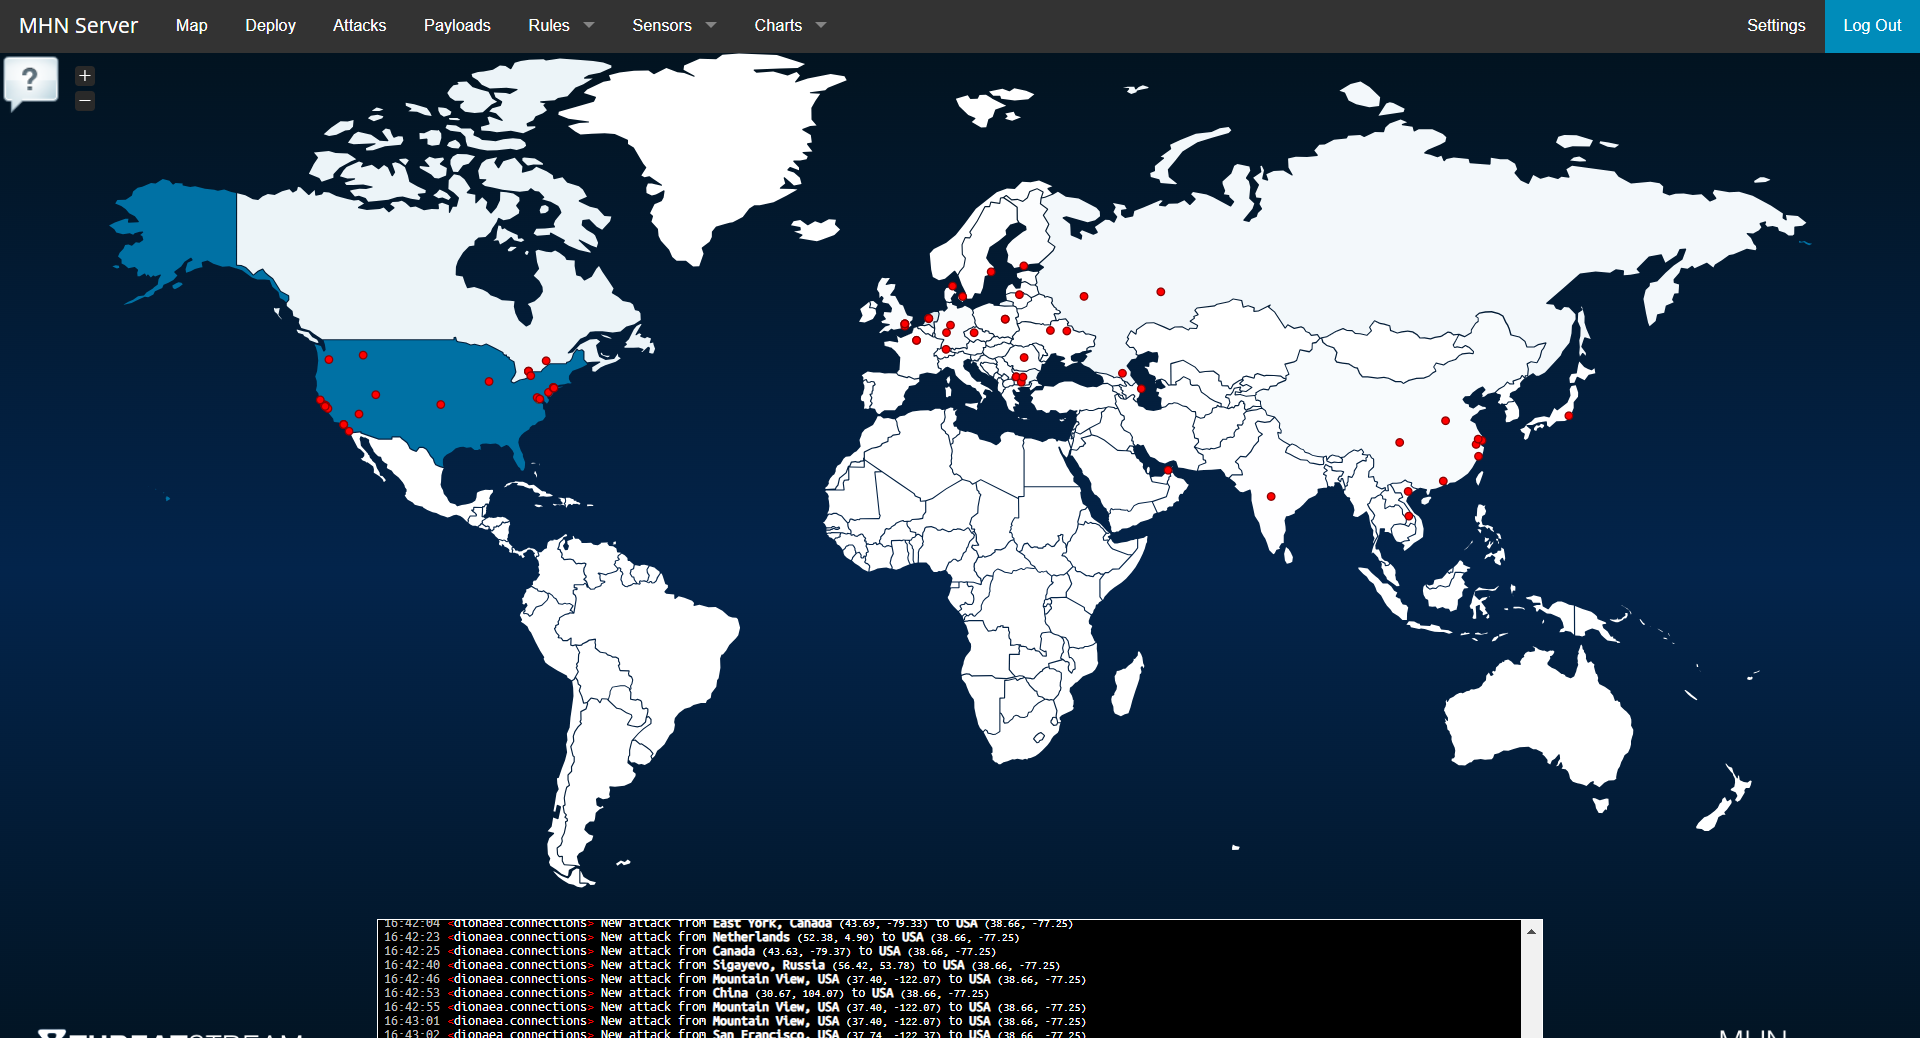
\includegraphics[width=\textwidth]{images/honeymap.png}
    \caption{Honeymap Output after about 50 mins}
    \label{fig:honeymap}
\end{figure}

Now, you can go to the \texttt{Deploy} page. Here, select, \texttt{Ubuntu/Raspberry Pi - Dionaea} under the dropdown and copy the command directly below it. An example of the page is shown in \reffig{fig:deploy}. This command will later be run in \textcolor{CornflowerBlue}{\texttt{mhn-honeypot}}.

\begin{figure}[h]
    \centering
    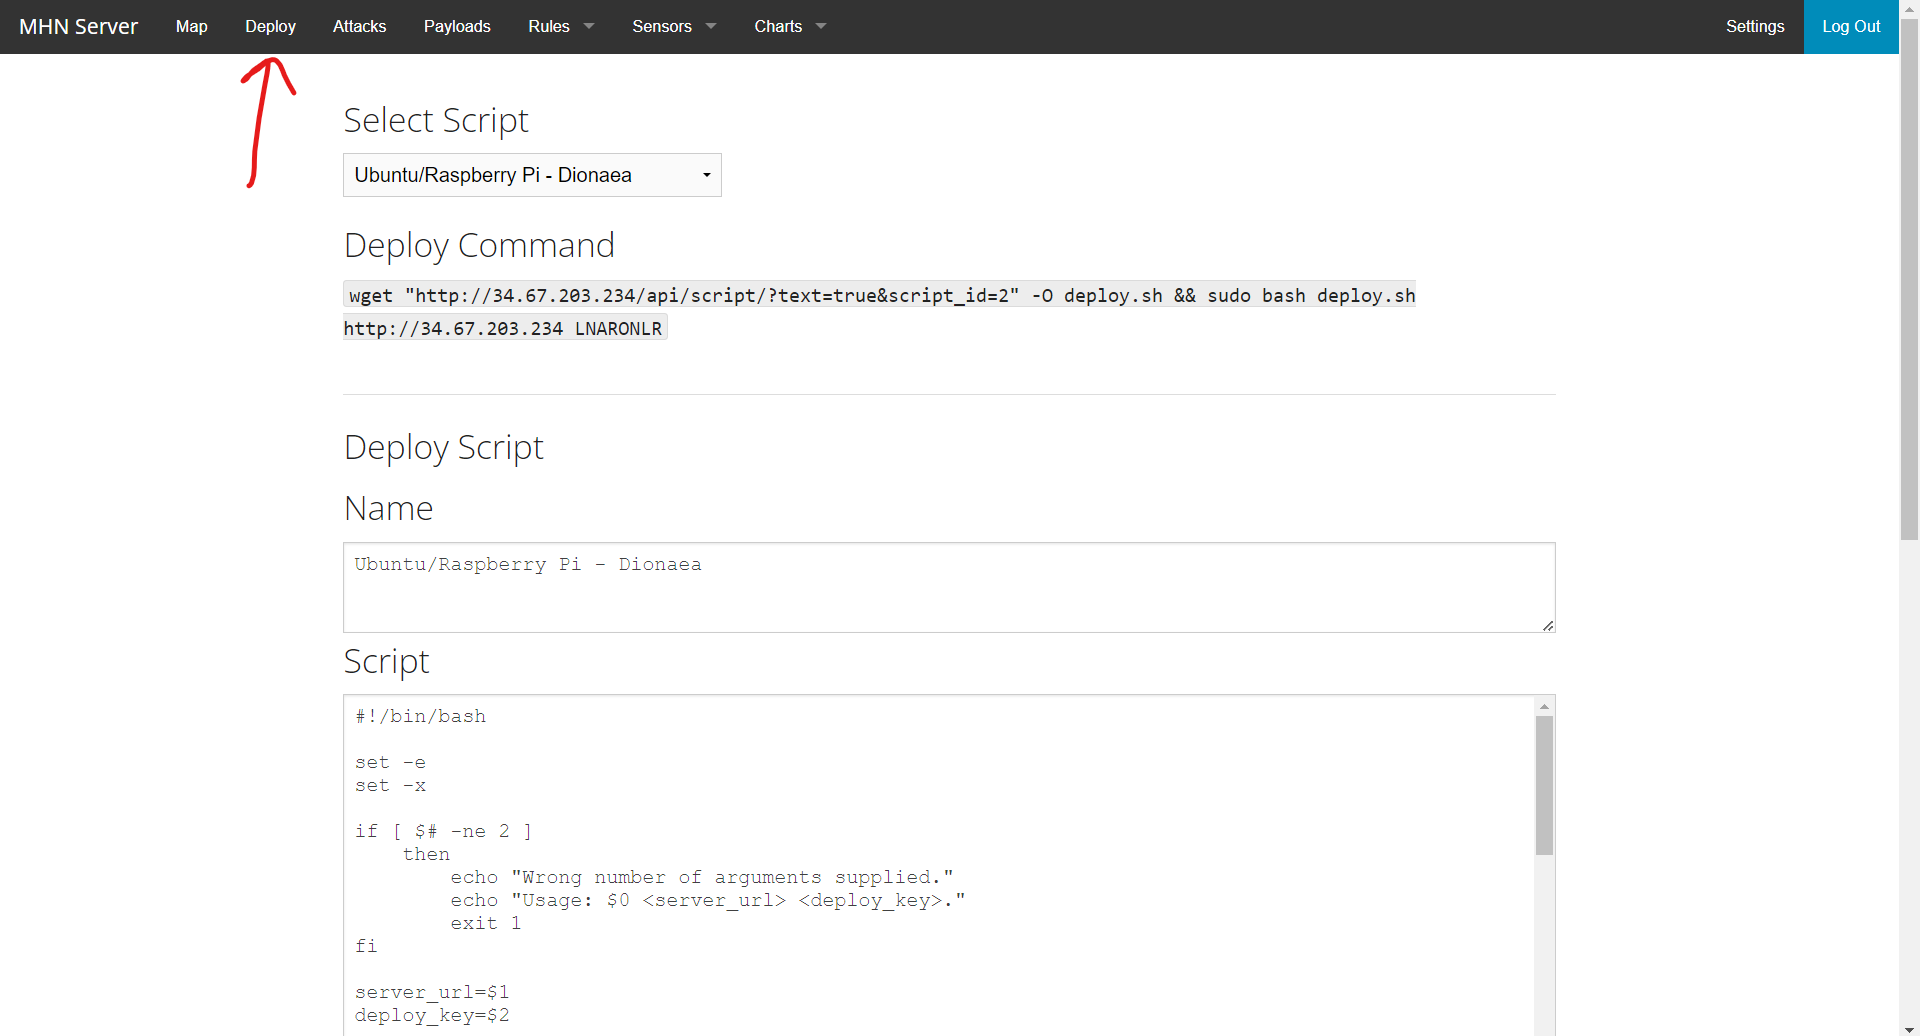
\includegraphics[width=\textwidth]{images/deploy.png}
    \caption{Deployment Page}
    \label{fig:deploy}
\end{figure}

Now, you can \texttt{exit} from the \textcolor{CarnationPink}{\texttt{mhn-admin}} VM and enter the \textcolor{CornflowerBlue}{\texttt{mhn-honeypot}} VM via SSH. Here, we need to first install \texttt{libemu-dev}, a package that is not, by default, installed in \texttt{Ubuntu 20.04}. Then, you can run the script you copied. This whole system is detailed in \refalgo{alg:dionaea}. With this, you have successfully deployed a honeypot. After a while, the honeymap (which is session-based) will start showing attacks coming from across the world on the map.

\begin{algorithm}[h]
\caption{Setup MHN Dionaea Honeypot}\label{alg:dionaea}
\begin{algorithmic}[1]
\State \texttt{sudo apt update}
\State \texttt{wget \url{http://archive.ubuntu.com/ubuntu/pool/universe/libe/libemu/libemu2_0.2.0+git20120122-1.2build1_amd64.deb} \url{http://archive.ubuntu.com/ubuntu/pool/universe/libe/libemu/libemu-dev_0.2.0+git20120122-1.2build1_amd64.deb}}
\State \texttt{sudo apt install ./libemu2\_0.2.0+git20120122-1.2build1\_amd64.deb ./libemu-dev\_0.2.0+git20120122-1.2build1\_amd64.deb} \Comment{Install \texttt{libemu-dev}}
\State \texttt{<copied command>}
\end{algorithmic}
\end{algorithm}

\section{Results} \label{sec-results}

We left Dionaea running for roughly a week, which gave us an incredibly large amount of data. This data is represented in \reffig{fig:choropleth} and \reffig{fig:heatmap} in the form of a choropleth and heatmap diagram respectively. The technologies \texttt{plotly} and \texttt{folium} were used for the creation of these figures.


\begin{figure}[h]
    \centering
    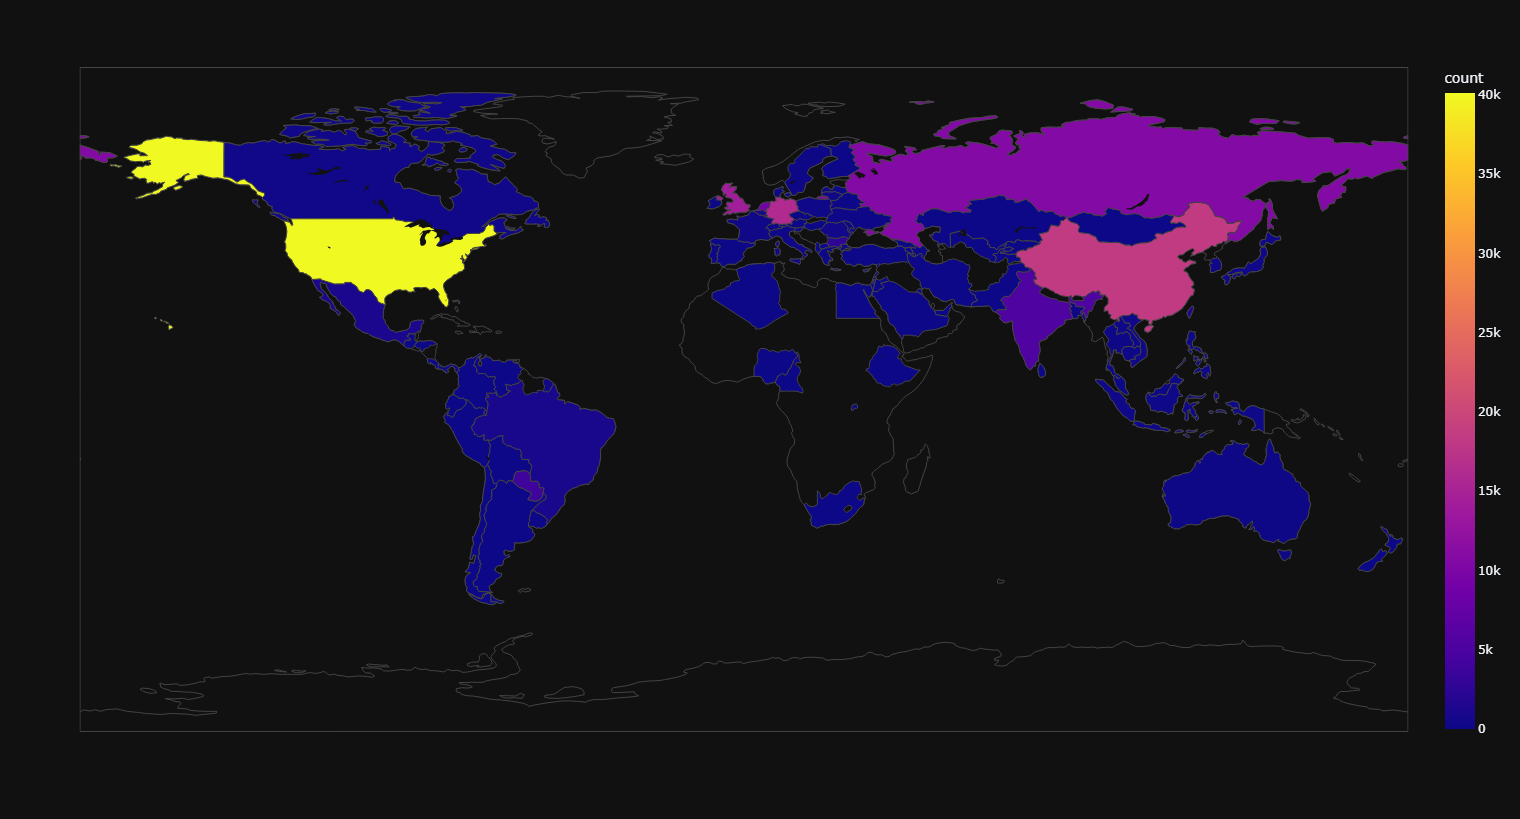
\includegraphics[width=\textwidth]{images/choropleth.png}
    \caption{Final Choropleth of Assembled Data}
    \label{fig:choropleth}
\end{figure}

\begin{figure}[h]
    \centering
    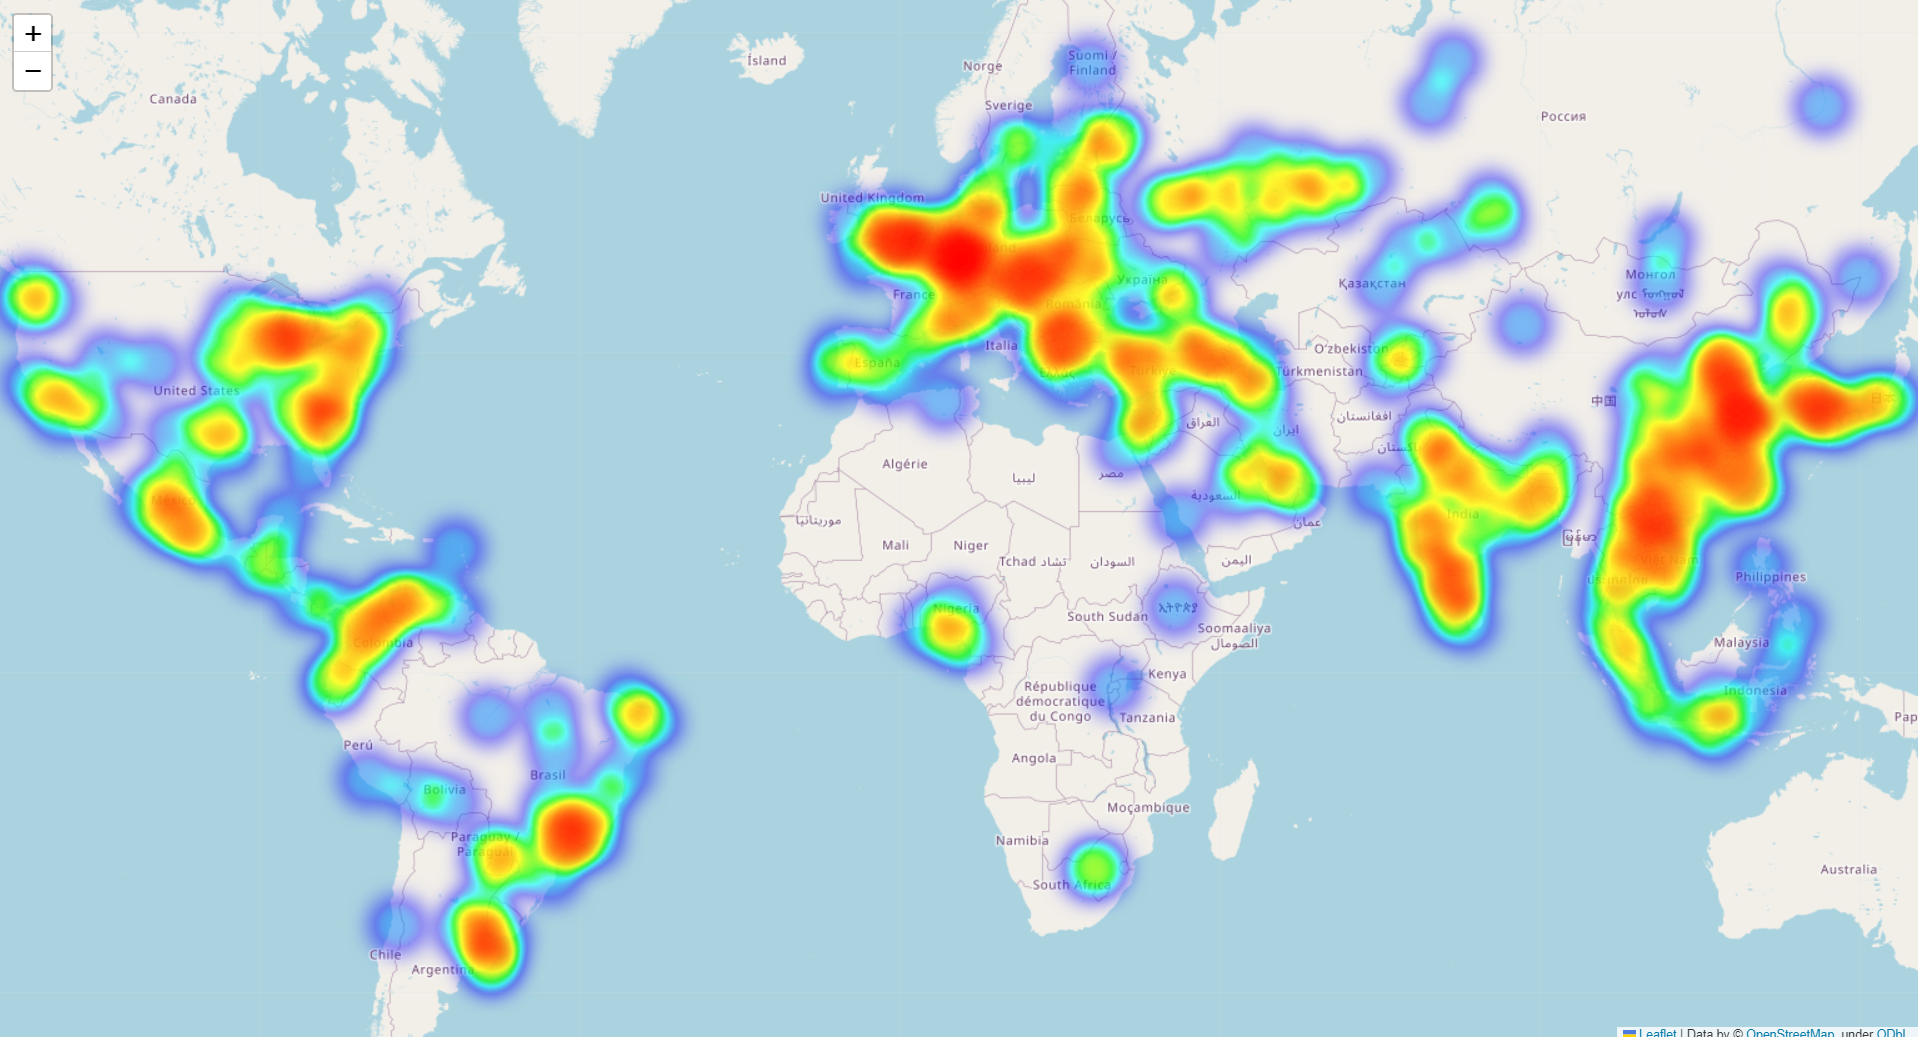
\includegraphics[width=\textwidth]{images/heatmap.png}
    \caption{Final Heat Map of Assembled Data}
    \label{fig:heatmap}
\end{figure}

We also aggregated several columns to get a better understanding. Notably, we had a huge number of attacks originating from the cities of \emph{Frankfurt am Main} in Hesse, Germany and \emph{Suqian} in Jiangsu, China. The attack from Germany occurred over roughly 20 minutes, whereas the attacks from China actually took roughly 9 hours. Neither of them used any form of malware, and hence no files were captured. Both attackers only attacked on the port \texttt{1900}. This suggests that they both used an automated software to attack, which resulted in similar numbers of attacks from both sides.

The top 10 locations to send IP addresses are illustrated in \reftable{tab:bigattacks}. We notice that ports \texttt{1900} and \texttt{445} were largely attacked. The attacks on port \texttt{1900} are likely a \href{https://www.cloudflare.com/learning/ddos/ssdp-ddos-attack/}{SSDP DDoS Attack}, where the attacker sends a lot of traffic in the form of a normal DDoS attack. The attacks from Frankfurt, Suqian and Hillsboro were likely of this kind. The attacks on port \texttt{445} is likely a form of \href{https://www.hackingarticles.in/smb-penetration-testing-port-445/}{SMB Penetration}, where the messages sent on TCP with port \texttt{445} are used to scan for vulnerabilities.

\begin{table}[h]
    \centering
    \begin{tabular}{cccc}
        \toprule \thead{Area of Origin} & \thead{Count} & \thead{Most Attacked Port} & \thead{Period of Attack} \\
        \midrule Frankfurt am Main, Hesse, Germany & 14,236 & Only attacked \texttt{1900} & 20 minutes \\
        Suqian, Jiangsu, China & 14,147 & Only attacked \texttt{1900} & 9 hours \\
        Ryazan', Ryazan Oblast, Russia & 5,901 & Attacked \texttt{445} 5,893 times & nearly 4 days \\
        Thiruvananthapuram, Kerala, India & 4,299 & Attacked \texttt{445} 4,277 times & 1 day \\
        Lima, San Pedro, Paraguay & 3,878 & Attacked \texttt{445} 3,876 times & 37 minutes \\
        Hillsboro, Oregon, USA & 3,687 & Only attacked \texttt{1900} & 52 minutes \\
        Shijiazhuang, Hebei, China & 1,462 & Attacked \texttt{445} 1,439 times & nearly 5 days \\
        Los Angeles, California, USA & 1,372 & Attacked 1,372 ports & 14 hours \\
        Mexico City, Mexico & 1,012 & Attacked \texttt{445} 1,010 times & 3 minutes \\
        \bottomrule
    \end{tabular}
    \caption{Largest Attacks as a Whole}
    \label{tab:bigattacks}
\end{table}

In terms of overall attacks from the countries, the largest number of attacks came from the USA, with 40,151 attacks. This far surpassed every other country's records. The rest of the records are shown at \reftable{tab:cntryattacks}.

\begin{table}[h]
    \centering
    \begin{tabular}{cccc}
        \toprule \thead{Country} & \thead{Count} & \thead{Most Attacked Port} & \thead{Main Attacking Region} \\
        \midrule USA & 40,151 & Attacked \texttt{1900} 3,726 times & South Carolina \\
        China & 18,470 & Attacked \texttt{1900} 14,152 times & Jiangsu \\
        Germany & 16,101 & Attacked \texttt{1900} 14,280 times & Hesse \\
        Great Britain & 14,162 & Attacked \texttt{10255} 122 times & England \\
        Russia & 10,773 & Attacked \texttt{445} 5,949 times & Ryazan Oblast \\
        Netherlands & 8,794 & Attacked \texttt{8080} 285 times & North Holland \\
        India & 5,349 & Attacked \texttt{445} 5,949 times & Kerala \\
        Paraguay & 3,884 & Attacked \texttt{445} 3,881 times & San Pedro \\
        Bulgaria & 2,657 & Attacked \texttt{9401} 12 times & Sofia-Capital \\
        \bottomrule
    \end{tabular}
    \caption{Attacks on the Country Scale}
    \label{tab:cntryattacks}
\end{table}


On the scale of the whole data sample, port \texttt{1900} was attacked 32,263 times and port \texttt{445} was attacked 18,695 times. The rest were much more miniscule in terms of scale.


Over the week-long period, we received 19 samples from various locations around the world. Dionaea made a certificate to access these files. We were unable to run them on the Cuckoo Sandbox due to limited resources. All of these samples were transferred in via a protocol known as \texttt{microsoft-ds}, which likely suggests these were Windows executables. Most of these samples originated from Vietnam and Indonesia.


\section{Conclusion} \label{sec-conclusion}

We conclude that a large portion of the attacks originate from the United States, which is not a surprise given the internet penetration rate in the country. This is closely followed by countries like China, Russia, Germany and India, which all too share this fact. By and large, this means that we have successfully created a preliminary proof-of-concept honeypot that received a total of 1500 attacks daily.


% \newpage 
% \section*{Acknowledgments} \noindent The author would like to thank NUS High School of Mathematics and Science for facilitating this project.

\section*{References}

\bibliographystyle{unsrt}
\bibliography{bib}

\end{document}

